% Класс документа пока не окончательный, сильно сомневаюсь, что article лучший
\documentclass[a4paper,12pt]{extarticle} 
% Подключаем шрифты,кодировки,русские переносы
\usepackage{cmap}
% подключается пакет, позволяющий улучшить вид пдф документа(как я понял)
\usepackage[T2A]{fontenc}
\usepackage[utf8x]{inputenc}
% подключаем кодировку шрифтов для вносимых файлов
\usepackage[main=russian,english]{babel}
% подключаем перенос и распознование слов, русский в приоритете
\usepackage{indentfirst}
% Отступ в начале абзаца
\usepackage{
	amssymb,
	amsfonts,
	amsmath,
}
% Пакеты американского математ. сообщества, красивый вид формул и текста внутри
\usepackage{
	wrapfig,
	graphicx,
	caption,
	subcaption,
	tikz,
}
% Обтекаемые объекты, рисунки, подписи и прочее
\usepackage{
	pgfplotstable,
	pgfplots,
	booktabs,
	colortbl,
	array
}
\pgfplotsset{compat=newest}
% таблицы, графики

\usepackage{xcolor}
\usepackage[unicode]{hyperref}

 % Цвета для гиперссылок
\definecolor{linkcolor}{HTML}{000000} % цвет ссылок
\definecolor{urlcolor}{HTML}{799B03} % цвет гиперссылок
\hypersetup{pdfstartview=FitH,  linkcolor=linkcolor,urlcolor=urlcolor, colorlinks=true}

\usepackage{geometry}
\usepackage{fancyhdr}
% границы, контитулы, и прочее


\geometry
	{
	left=2.2cm,
	right=2.2cm,
	bottom=2cm,
	top=2cm,
	}
% границы документа

\usepackage{setspace}
% убирает гигантские размеры оглавления
\linespread{1.3}
% междустрочный интервал

\pagestyle{fancy}
\fancyhead{}
% пустая шапка контитула
\fancyhead[R]{\authors}
% На правой стороне страницы авторы и науч.рук.
\fancyhead[L]{\shortlabname}
 % Слева название лабы
\fancyfoot{}
\fancyfoot[C]{\thepage}
% номер страницы снизу по середине
\renewcommand{\contentsname}{Оглавление}
% переводим на русский язык оглавление
\usepackage{secdot}
\sectiondot{subsection}
% Ставит злосчастные точки в главах, ибо не по госту
% Преамбула почти слизана у Федора Сарафанова https://github.com/FedorSarafanov/RLC/blob/master/text/diss.tex

	\def\authors{Есюнин М.В., Есюнин Д.В.}
	\def\labname{Электромагнитное экранирование}
	\def\sciadviser{Павличенко И.А.}
	\def\shortlabname{Электромагнитное экранирование}
\usepackage{float}
\begin{document}
\begin{titlepage}

\begin{center}

	\textsc{Нижегородский государственный университет имени Н.\,И. Лобачевского}
	\vskip 4pt \hrule \vskip 8pt
	\textsc{Радиофизический факультет}

	\vfill

	{\Large\labname}

\end{center}

\vfill

\begin{flushright}
	{Работу выполнили студенты\\ \authors\\ 430 группы\\ \vskip 14pt преподаватель:\\ \sciadviser}
\end{flushright}

\vfill

\begin{center}
	Нижний Новгород, \the\year
\end{center}

\end{titlepage}
% \renewcommand{\vec}{\mathbf}

\renewcommand{\phi}{\varphi}
\renewcommand{\hat}{\widehat}

\tableofcontents

\newpage
\sloppy

\section{Цели работы}
Настоящая работа преследует следующие две основные цели.
\begin{itemize}
	\item Экспериментальное наблюдение явления экранирования переменного магнитного поля металлическими оболочками и выяснение роли основных физических факторов, определяющих степень проникновения поля через экран; к числу таких факторов относятся: свойства материала экрана (проводимость и магнитная проницаемость), толщина его стенок, частота поля.
	\item Теоретический расчет экранирующих свойств металлических оболочек на простой модели и сопоставление экспериментальных и теоретических данных.
\end{itemize}
\section{Элементы теории}
\subsection{Основные понятия}
Под электромагнитным экранированием понимается изоляция некоторой области пространства от проникновения электромагнитных полей, существующих в соседних областях. В статических или переменных квазистационарных полях (которым соответствуют длины волн, много большие характерных размеров используемых приборов и устройств) такая изоляция осуществляется обычно с помощью замкнутых металлических оболочек - экранов. Явление экранирования поля проводящими оболочками имеет большое практическое значение. В частности, оно широко используется в электро- и радиотехнике для уменьшения паразитных связей между различными элементами приборов. В некоторых случаях, напротив, может возникнуть необходимость принимать специальные меры для борьбы с этим явлением.
Общей физической причиной ослабления поля внутри 
экрана является то обстоятельство, что наведенные в нем внешним полем токи (или заряды) создают во внутренней области поле, противоположное внешнему. В результате суммарное поле в этой области, складывающееся из нолей внешних и наведенных источников, уменьшается.

\subsection{Расчет экранирующего действия металлических
оболочек}

В качестве экранов в работе используются оболочки цилиндрической формы. Строгий расчет их экранирующего действия представлял бы собой весьма сложную задачу, требующую использования численных методов. Однако для получения качественных оценок, ослабления поля в экранированной области и установления общего характера его зависимости от параметров можно ограничиться изучением более простых моделей, допускающих точное решение задачи в известных аналитических функциях. Моделями такого рода являются, например, плоский, цилиндрический и сферический слои. Поскольку высота и диаметр внутренней полости используемых в работе цилиндров одинаковы и весьма малы по сравнению с длиной волны в свободном пространстве $\lambda_0$, наиболее адекватной моделью, по-видимому, следует считать сферический слой, который имеет тот же объем внутренней полости и внешний радиус $a \ll \lambda_0$. Последнее условие означает, что вне металла (т.е. как во внешней, так и в экранируемоей областях) поле можно рассматривать как квазистатическое.
Если замкнутая однородная сферическая оболочка помещена в квазистатическое внешнее поле с комплексным вектором напряженности $\vec{H}_{0} e^{i \omega t}$, которое в ее отсутствие является однородным, то поле в ограничиваемой ею области $\vec{H}_{1} e^{i \omega t}$ также однородно. Эффективность экранирования удобно характеризовать величиной отношения комплексных амплитуд этих полей:
\begin{equation} 
\eta_{m}=H_{0} / H_{1}
\label{eq:1}
\end{equation}
Величина $|\eta_{m}|$ показывает, в какое число раз ослабляется поле в экранированной области, и может быть названа коэффициентом ослабления. Она, естественно, сильно зависит от соотношения между толщиной экрана $d$ и толщиной скин-слоя $\delta=c/(2\pi\sigma\mu\omega)^{\frac{1}{2}}$ ($c$ - скорость света в вакууме, $\sigma$ - проводимость, $\mu$ - магнитная проницаемость экрана). В двух предельных случаях ($\delta \ll d$  и $\delta \gg d$) выражение для $\eta_{m}$(в общем случае довольно громоздкое) существенно упрощается и при выполнении дополнительного условия $d \ll a$ принимает следующий вид:

\begin{enumerate}
	\item $\delta \ll d$ (сильный скин-эффект):
	\begin{equation} 
		\eta_{m}=\frac{1}{6}\left[(1-i) \frac{\mu \delta}{a}+3+(1+i) \frac{a}{\mu \delta}\right] \exp \left[(1+i) \frac{d}{\delta}\right]
	\label{eq:2}
	\end{equation}
При $\mu=1$
\begin{equation} 
	\eta_{m}=\frac{1}{6}(1+i) \frac{a}{\delta} \exp \left[(1+i) \frac{d}{\delta}\right]
\label{eq:3}
\end{equation}

	\item $\delta \gg d$ (скин-эффект отсутствует):
	\begin{equation}
		\eta_{m}=1+\frac{2}{3}\frac{d}{a}\frac{(\mu-1)^2}{\mu}+i\frac{2}{3}\frac{ad}{\mu \delta^2}
	\label{eq:4}
	\end{equation}
При $\mu=1$
\begin{equation} 
\eta_{m}=1+i \frac{2 a d}{3 \delta^{2}}
\label{eq:5}
\end{equation}
\end{enumerate}

Для приближенных оценок величины $\eta_{m}$ (с точностью $\sim10\%$) выражения \eqref{eq:2}—\eqref{eq:5} можно использовать и в промежуточном случае ($\delta \simeq d$), разграничивая области применимости формул \eqref{eq:2}, \eqref{eq:3}, с одной стороны, и \eqref{eq:4}, \eqref{eq:5}, с другой стороны, точкой $\delta = d$.

Заметим, что приведенные результаты расчета позволяют описать также экранирующее действие сферической металлической оболочки по отношению к переменному электрическому полю. В частности, при $\delta \gg a$ выражение для комплексного коэффициента ослабления электрического поля $\eta_{\varepsilon}$, легко получается на основании принципа перестановочной двойственности из выражения \eqref{eq:4} путем замены в нем магнитной проницаемости $\mu$ на диэлектрическую проницаемость проводника $\varepsilon=4\pi \sigma / i \omega$. В диапазоне радиочастот величина $|\varepsilon|$ для хороших проводников и определяемая ею величина $|\eta_{\varepsilon}|$ принимают чрезвычайно высокие значения, недоступные для измерений в условиях настоящей работы даже при весьма малой толщине экранов. Например, при $d/a \simeq 10^{-3}, \sigma \simeq 10^{17} c^{-1}, \omega \simeq 10^{4} c^{-1}$, пренебрегая в \eqref{eq:4} малыми членами и заменяя $\mu$ на $\varepsilon$, получаем:
\begin{equation} 
	\eta_{\varepsilon}=2 \varepsilon d / 3 a=-i 8 \pi \sigma d / 3 \omega a \simeq-i \cdot 10^{11}
\end{equation}
В полном соответствии с законами электростатики при $\omega\rightarrow 0 $ величина $\eta_{\varepsilon} \rightarrow \infty $, т.е. электрическое поле внутрь экрана не проникает.
\section{Описание экспериментальной установки}
\begin{figure}[h]
	\centering
	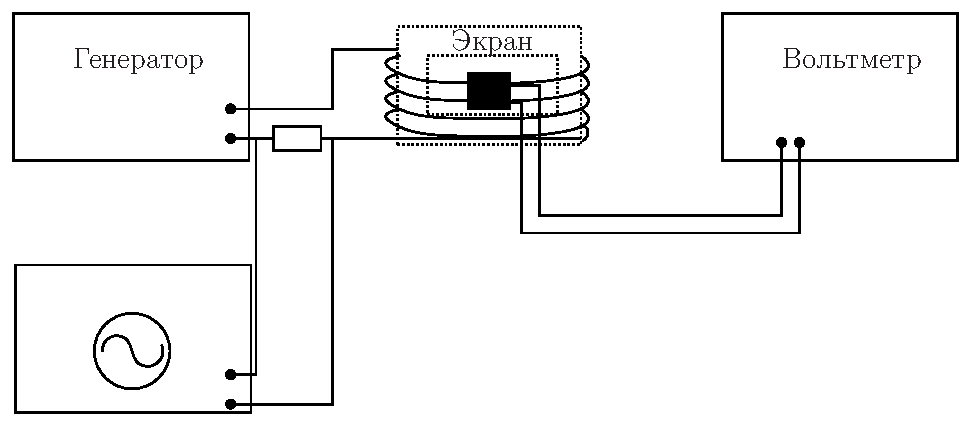
\includegraphics[scale=1]{text/main2.pdf}
	\caption{Схема экспериментальной установки}
	\label{fig:figure1}
\end{figure}
Лабораторная установка предусматривает проведение измерений коэффициентов ослабления для трех латунных и трех стальных экранов цилиндрической формы. Внутренние размеры всех цилиндров одинаковы (высота $h$ = 50мм, диаметр основания $D$ = 50мм), а толщина стенок различна (2мм, 5мм, 10мм). Значения проводимости $\sigma$ и магнитной проницаемости $\mu$ латуни и стали приведены ниже (в гауссовой системе единиц).
Латунь: $\sigma \simeq 1.5\cdot 10^{17} c^{-1}, \mu \cong 1$.
Сталь: $\sigma \simeq 0.7\cdot 10^{17} c^{-1}, \mu \sim 10^2 \div 10^3 $ (при $H \sim 10\text{ }$ эрстед).
Схема измерения коэффициента ослабления магнитного поля изображена на рисунке \ref{fig:figure1}. Переменное магнитное поле создается внутри соленоида, подключенного к выходу звукового генератора. В качестве индикатора ноля используется второй соленоид (меньших размеров), с выхода которого переменное напряжение может подаваться на усилитель вольтметра. Надевая больший (генераторный) соленоид сначала на открытый (неэкранированный) индикатор, а затем на индикатор, закрываемый экраном, и измеряя, как изменяются при этом показания вольтметра, мы могли бы (при неизменности амплитуды тока в цепи внешнего соленоида) определить тем самым коэффициент ослабления $|\eta_{\mu}|$. Поскольку, однако, внесение металлического экрана внутрь внешнего соленоида, вообще говоря, изменяет его коэффициент самоиндукции, а следовательно, и его импеданс, сила тока в цепи внешнего соленоида и создаваемое этим током магнитное поле $H_0$ при наличии экрана и в его отсутствие могут быть различными. Это необходимо учитывать при определении величины $|\eta_{\mu}|$. В используемой схеме предусмотрено измерение относительных изменений токов как во внутреннем, так и во внешнем соленоидах. С этой целью в цепь внешнего соленоида введено сопротивление $R$, напряжение с которого подается на вертикальный усилитель осциллографа. Величина $|\eta_{\mu}|$ должна определяться по формуле:
\begin{equation}
	|\eta_{\mu}|=\frac{V_0U_e}{V_eU_0}
\label{eq:7}
\end{equation}
где $V$ и $U$ - соответсвенно показания вольтметра и осциллографа, индексы $0$ и $e$ относятся соответственно к величинам измеренным без экрана и с экраном.
\section{Практическая часть}
\subsection{Задания 1,2}
Для каждого экрана(латунь, сталь) сняли экспериментальную зависимость коэффициента ослабления магнитного поля $|\eta_{\mu}|$ от частоты $f$.
\begin{figure}[H]
	\vspace{-15pt}
	\centering
	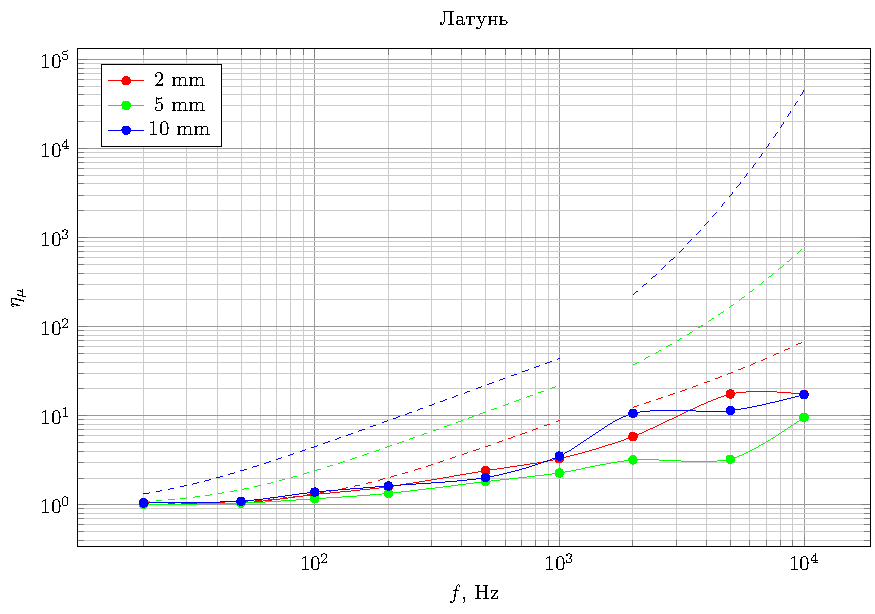
\includegraphics[scale=1]{plots/Lat.pdf}
	\caption{Теоретическая зависимость $|\eta_{\mu}(f)|$ указана пунктиром.}
	\label{fig:figure2}
	\vspace{-20pt}
\end{figure}
\begin{figure}[H]
	\vspace{-10pt}
	\centering
	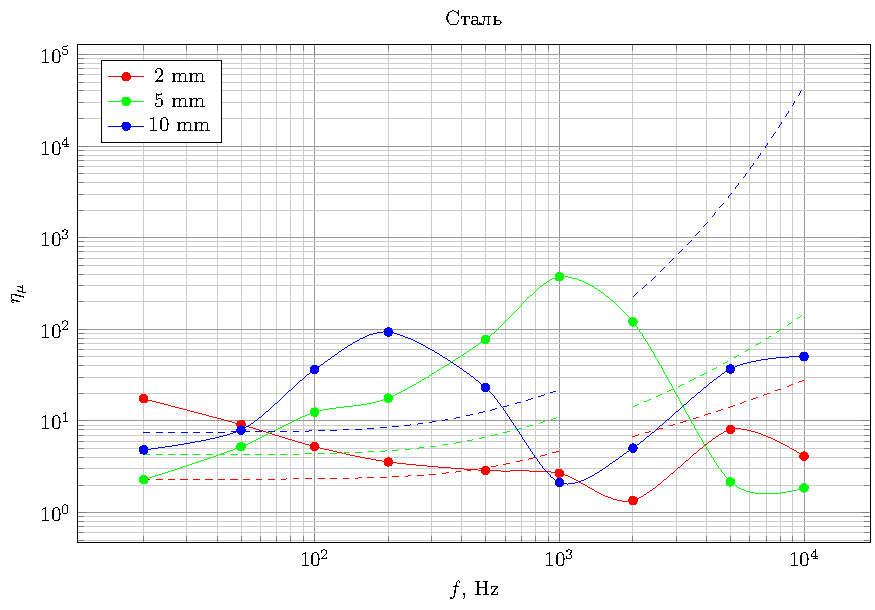
\includegraphics[scale=1]{plots/Steel.pdf}
	\caption{Теоретическая зависимость $|\eta_{\mu}(f)|$ указана пунктиром.}
	\label{fig:figure3}
	\vspace{-10pt}
\end{figure}
Принимая в качестве модели цилиндрического экрана сферический слой той же толщины $d$ и с тем же объемом внутренней полости $V=(4\pi/3)(a-d)^3=\pi R^2h$ (отсюда, ввиду $a\gg d$, имеем $a\cong (3R^2h/4)^{1/3}$), построили для исследуемых экранов графики теоретической зависимости $|\eta_{\mu}(f)|$.

Качественное совпадение наблюдается в области малых частот(до 1000 Hz). Для более высоких частот теория от эксперимента отличается в 20 порядков.
\subsection{Задание 3}
Используя результаты измерений для стальных экранов, рассчитали приблизительно на основании той же сферической модели для случая $\delta (f) \ll d$ (формула \eqref{eq:2}) значения магнитной проницаемости стали $\mu$. Способ приближенного расчета состоял в численном решение уравнения для 3 нижних частот (для высоких частот модель \textbf{не совпадает}) частот и последующем усреднении результатов.
\begin{table}[htbp]
  \centering
  \caption{Магнитная проницаемость $\mu$ для разных частот $f$ и толщины экрана $d$}
    \begin{tabular}{|c|c|c|c|}
    \toprule
    $f$, Hz & $\mu$, 2mm & $\mu$, 5mm & $\mu$, 10mm \\
    \midrule
    20 & 306.25 & 13.05 & 18.64 \\
    \midrule
    50 & 179.35 & 38.76 & 32.26 \\
    \midrule
    100 & 94.83 & 102.01 & 146.13 \\
    \midrule
    $\langle \mu \rangle$ & 193.48 & 51.27 & 65.68 \\
    \bottomrule
    \end{tabular}%
\end{table}%
По полученным данным можно сделать вывод о недостаточной точности эксперимента. Хотя качественно $\mu$ для стали действительно лежит в пределах $100-1000$.
\section{Вывод}
\begin{enumerate}
	\item Экспериментально наблюдали явление экранирования переменного магнитного поля металлическими оболочками и выяснили роль основных физических факторов, определяющих степень проникноваения поля через экран
	\item Теоретически расчитали экранирующие свойства металлических оболочек на простой модели и сопоставили экспериментальные и теоретические данные.
	\begin{itemize}
		\item В области малых частот простая модель действительно хорошо описывает экранирующие свойства цилиндрического экрана. В области высоких частот теория модели отличается на несколько порядков, что говорит о неприменимости модели.
		\item Для стали магнитная проницаемость варьируется в достаточно широких пределах. Это говорит о том, что необходимо повысить чувствительность эксперимента для более точного определения $\mu$.
	\end{itemize}
\end{enumerate}
\end{document}